% !TeX TS-program = xelatex

\documentclass[10pt]{beamer}

\usepackage{color, colortbl}
\usetheme[progressbar=frametitle]{metropolis}
\usepackage{appendixnumberbeamer}
\usepackage{pgfplots}
\usepackage{xspace}
%\usepackage{listings}
%\usepackage{minted}
\usepackage{graphics}

\usepackage{tabularray}

\usepackage{pifont}% http://ctan.org/pkg/pifont

%\definecolor{lgrey}{rgb}{220,220,220}
%
%
%
%\usepackage{fontspec}
\newfontfamily{\FA}{FontAwesome.otf}
%
%
%\usepackage{fontawesome}

\newcommand{\bluecheck}{{\color{green}\checkmark}}

\usepackage{makecell}
%\newcommand{\bluecross}{{\color{green}\checkmark}}
\newcommand{\xmark}{\ding{55}}%

\newcommand{\bluecross}{{\color{red}\xmark}}

\usepackage{tikz}
\usetikzlibrary{positioning}



\usepackage{tabularx}


\newcommand\blfootnote[1]{%
	\begingroup
	\renewcommand\thefootnote{}\footnote{#1}%
	\addtocounter{footnote}{-1}%
	\endgroup
}

%\usepackage{fontspec}
%\newfontfamily{\FA}{FontAwesome.otf}



\newcommand{\themename}{\textbf{\textsc{metropolis}}\xspace}


\newcommand\extrafootertext[1]{%
	\bgroup
	\renewcommand\thefootnote{\fnsymbol{footnote}}%
	\renewcommand\thempfootnote{\fnsymbol{mpfootnote}}%
	\footnotetext[0]{#1}%
	\egroup
}



%
%\setsansfont[BoldFont={Fira Sans}]{Fira Sans Light}
%\setmonofont{Fira Mono}
%\usepackage[sfdefault]{Fira Sans}

\title{ANC of mains power interference in CW searches}
\subtitle{}

\author{\textbf{Tom Kimpson}, \\ S. Suvorova, H.Middleton, C.Liu,  A. Melatos, R. Evans, and W. Moran}



\date{\textit{LIGO CW working group, November 8, 2023}}



%\titlegraphic{\hfill
\includegraphics[height=1.5cm]{images/logo}}



\titlegraphic{%
	\begin{picture}(0,0)
		\put(105,-210){\makebox(0,0)[rt]{
\includegraphics[width=3cm]{images/unimelb_logo_2}}}
	\end{picture}
	\begin{picture}(0,0)
		\put(305,-200){\makebox(0,0)[rt]{
\includegraphics[width=3cm]{images/logo	}}}
\end{picture}



}



\begin{document}
	
	\maketitle
	
	\begin{frame}{Summary}
		
		\metroset{block=fill}
		\begin{block}{\alert{Takeaway points}}
			\begin{itemize}
				\item Instrumental lines hamper CW searches.
				\item It is possible to subtract lines using adaptive noise cancellation (ANC) 
				\item ... if there is reference data from a PEM
				\item ANC + HMM search on synthetic data can recover CW signal which overlaps with mains power interference at 60 Hz
			\end{itemize}
		\end{block}
		
	\end{frame}


\begin{frame}{Instrumental lines}
	\centering
	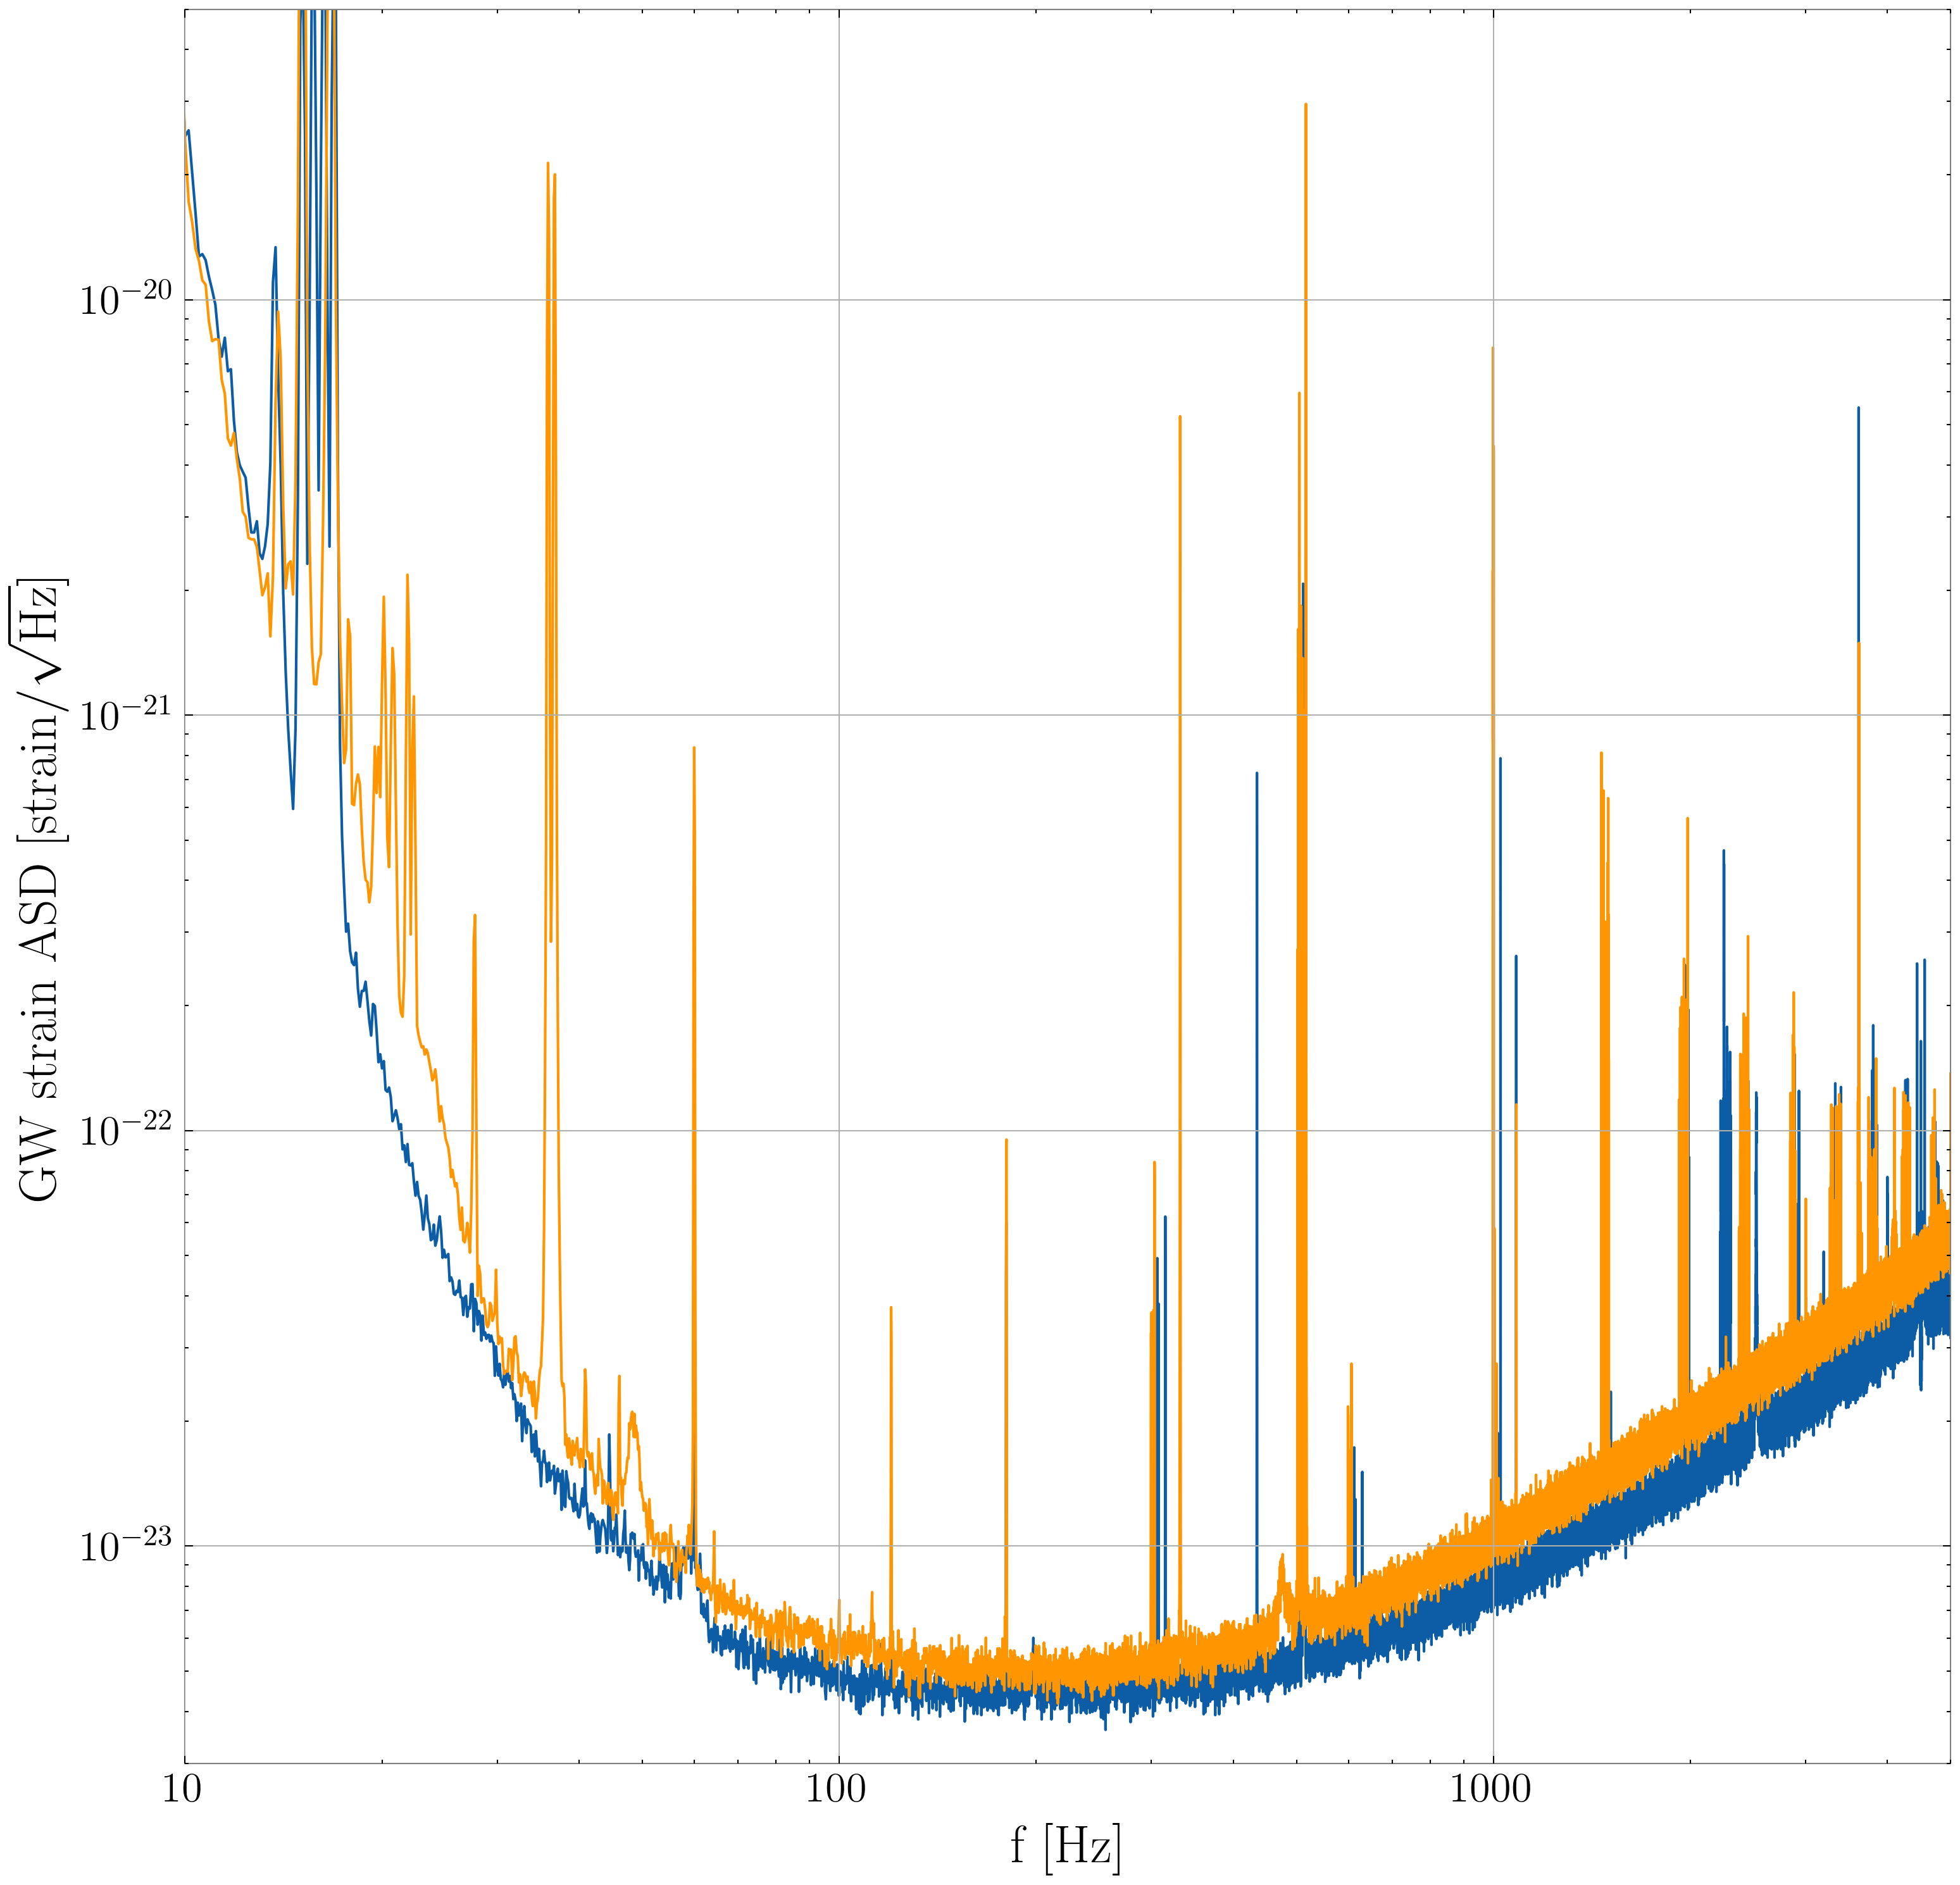
\includegraphics[width=0.8\textwidth,height=0.7\textwidth]{images/sensitivity_sq}
%	\extrafootertext{channel \texttt{*:DCS-CALIB\_STRAIN\_C01\_AR}}
	
	
\end{frame}


	
%\begin{frame}{Instrumental lines}
%	
%	\begin{itemize}
%		\item Lines = long-lived, narrowband spectral artefacts 
%		\item Origin = electrical subsystems, mechanical subsystems
%		\item Lines are disruptive for CW searches. Spectrally, a quasi-monochromatic GW source $\approx$ instrumental line.
%	\end{itemize}
%	
%
%%	\extrafootertext{A log of lines is maintained at: dcc.ligo.org/LIGOT2100200/public}
%	
%	
%\end{frame}




\begin{frame}
	
	\raggedright
	Some lines are static, but some are wandering: 
	
	\centering
	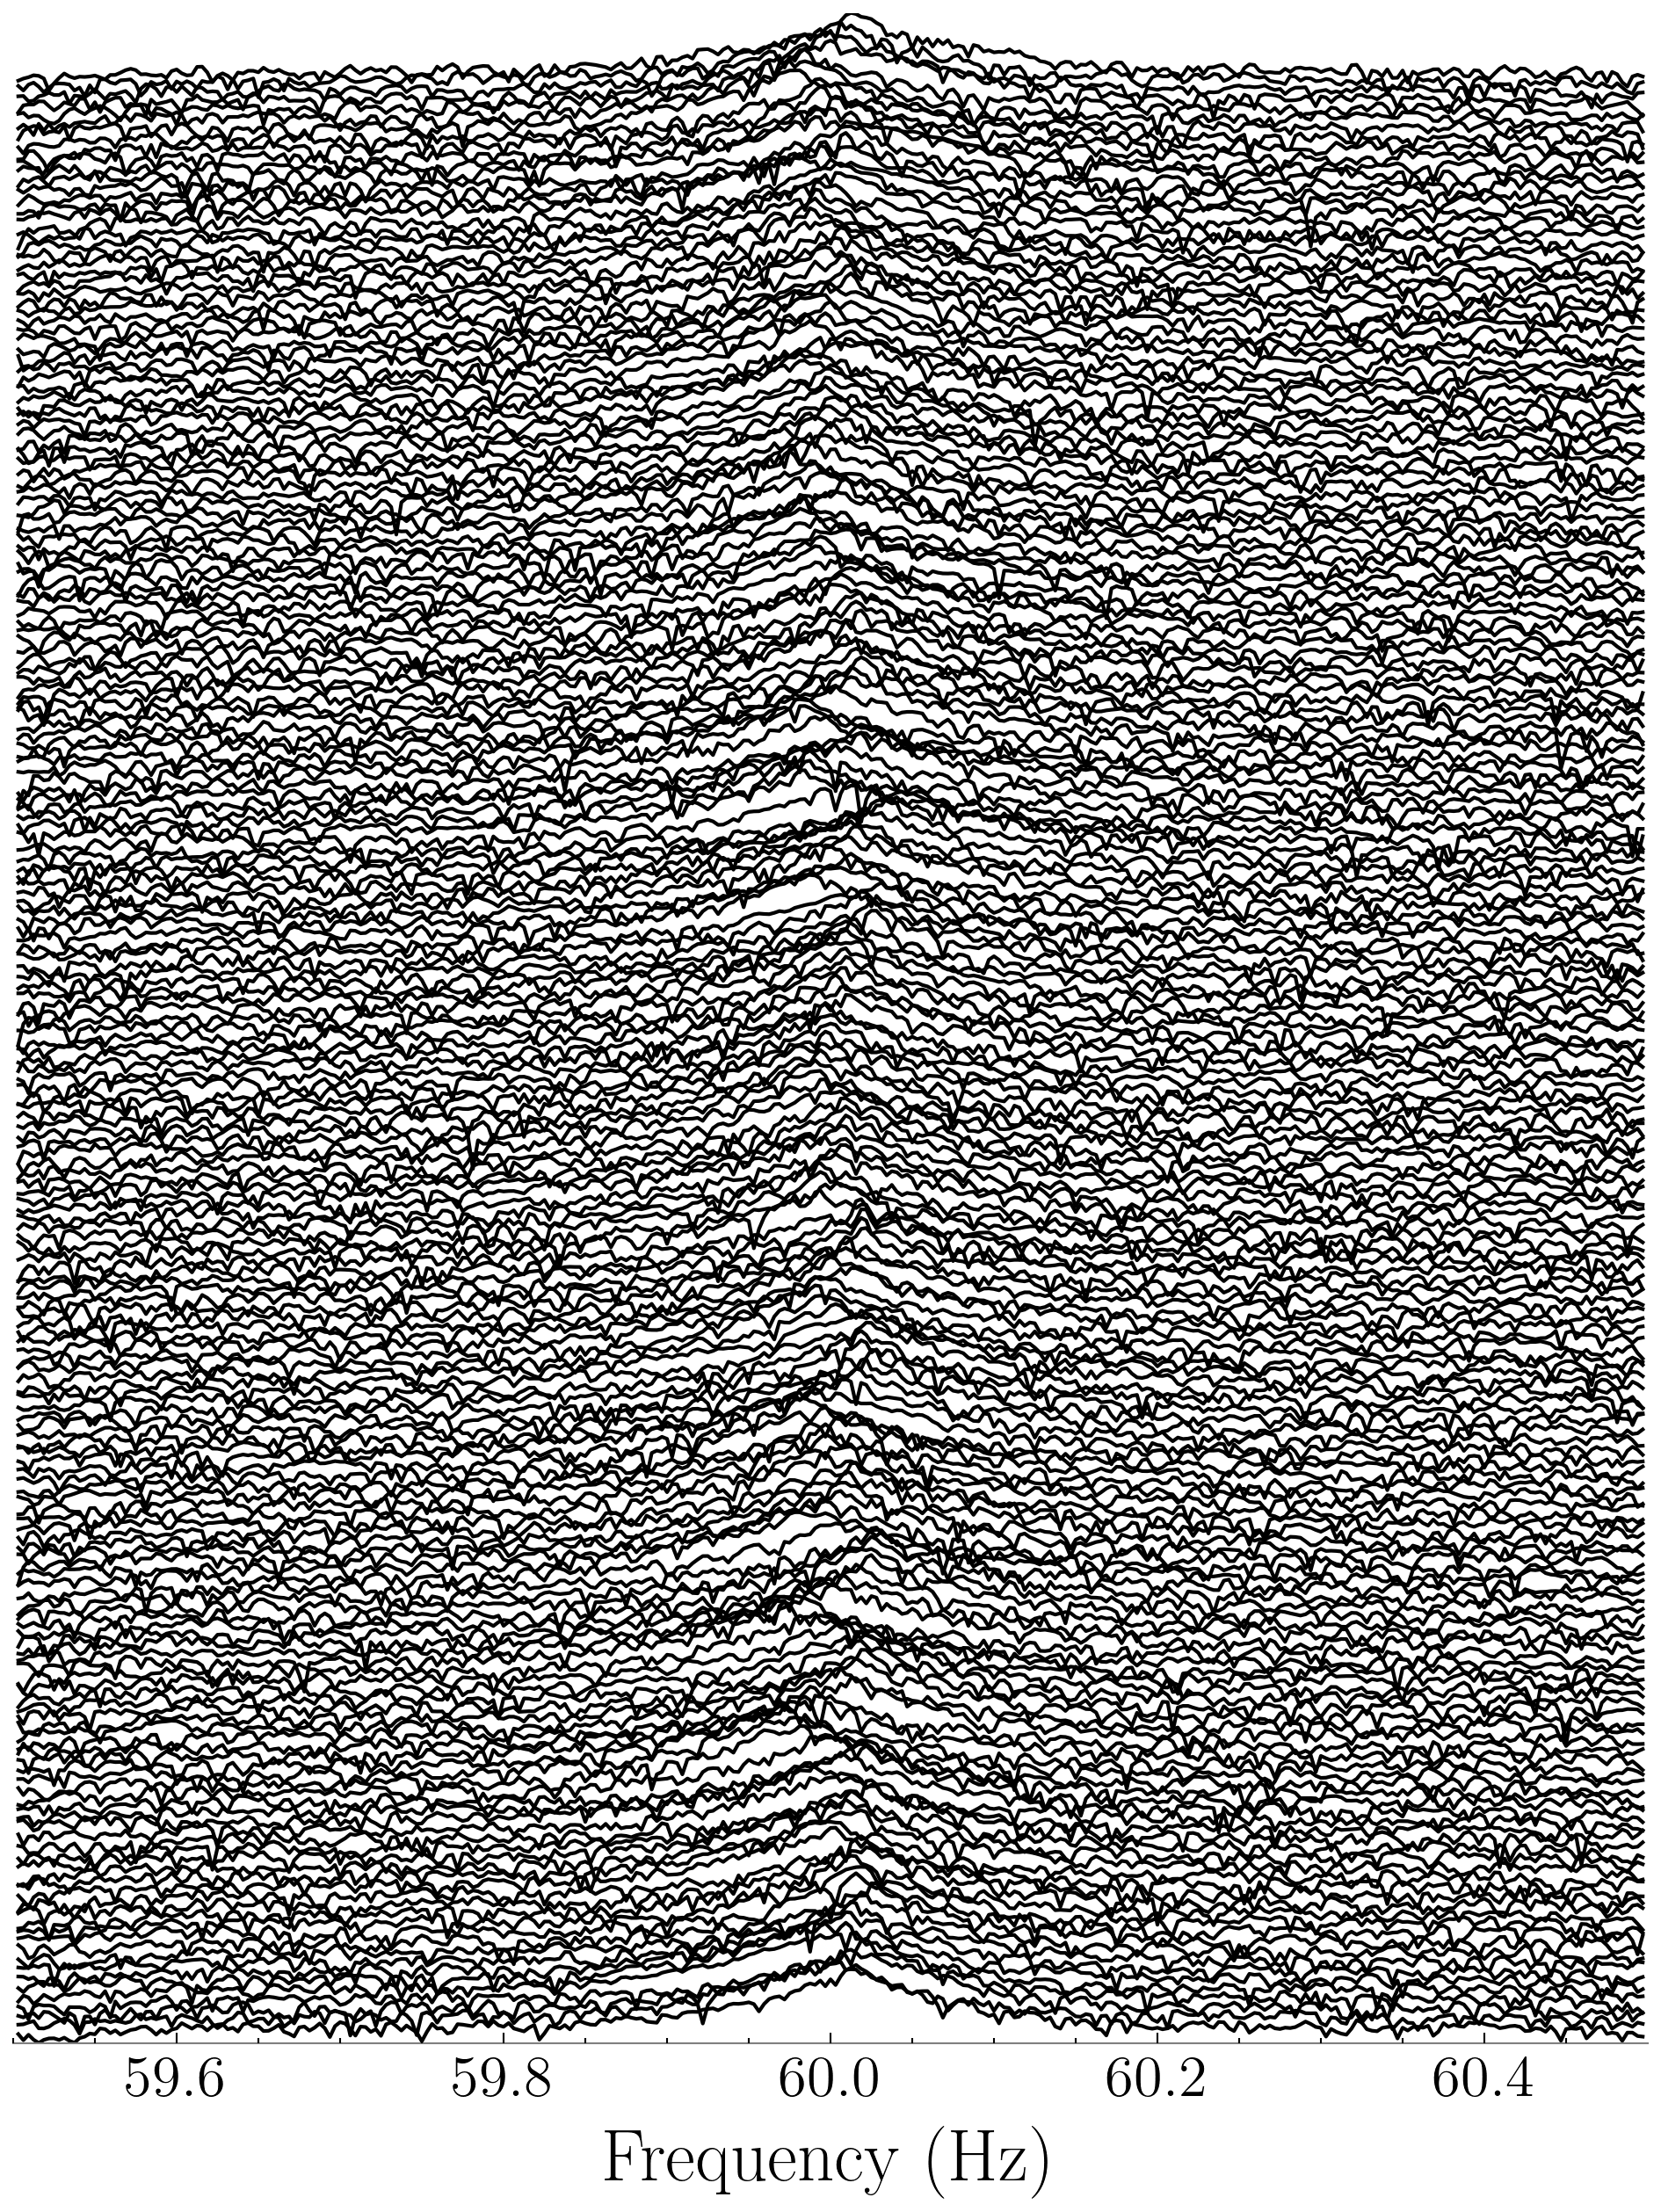
\includegraphics[width=0.53\textwidth,height=0.7\textwidth]{images/new_cascade_O3_new}
	
\extrafootertext{channel \texttt{H1:PEM-CS\_MAINSMON\_EBAY\_1\_DQ}}
	
	
\end{frame}




\begin{frame}
	

		\begin{itemize}
			\item How do we typically deal with lines?
			\begin{itemize}
				\item Veto candidates / gate frequency bands
			\end{itemize} 
			
			\item \alert{This work:} can we detect a synthetic CW signal that overlaps with a line? 
			\begin{itemize}
					\item We focus exclusively on the \alert{60 Hz line} (North America power grid) 
			\end{itemize}
			

		\end{itemize}
		
			
\end{frame}







\begin{frame}{ANC}
	
We can subtract the line ``\alert{clutter}'' using adaptive noise cancellation (ANC). 
	
\begin{itemize}
	\item Signal channel: $x(t) = h(t) + \alert{c(t)} + n(t)$
	\item Reference channel: $r\,(t)$
	\item Use $r\,(t)$ to construct real-time estimate $\hat{c}\,(t)$ via an \textbf{adaptive} filter
	\item Define a ``residual'' $e(t) = x(t) - \hat{c}(t)$
	\item As $\hat{c}\,(t) \to c(t)$, $e(t) \to h(t) + n(t)$
\end{itemize}	

Analogous to how your noise cancelling headphones work.

\end{frame}


\begin{frame}
	
	
	
	\begin{columns}
		\column{0.4\textwidth}
		
		\begin{itemize}
			\item Where does our $r\,(t)$ come from? 
			\begin{itemize}
				\item PEMs
			\end{itemize}
			\item There are 9 PEM mains voltage monitors:
			\begin{itemize}
				\item 3 $\times$ \texttt{EX}
				\item 3 $\times$ \texttt{EY}
				\item 3 $\times$ \texttt{CS}
			\end{itemize} 
		\end{itemize}
		
		
	
		\column{0.6\textwidth}
		
		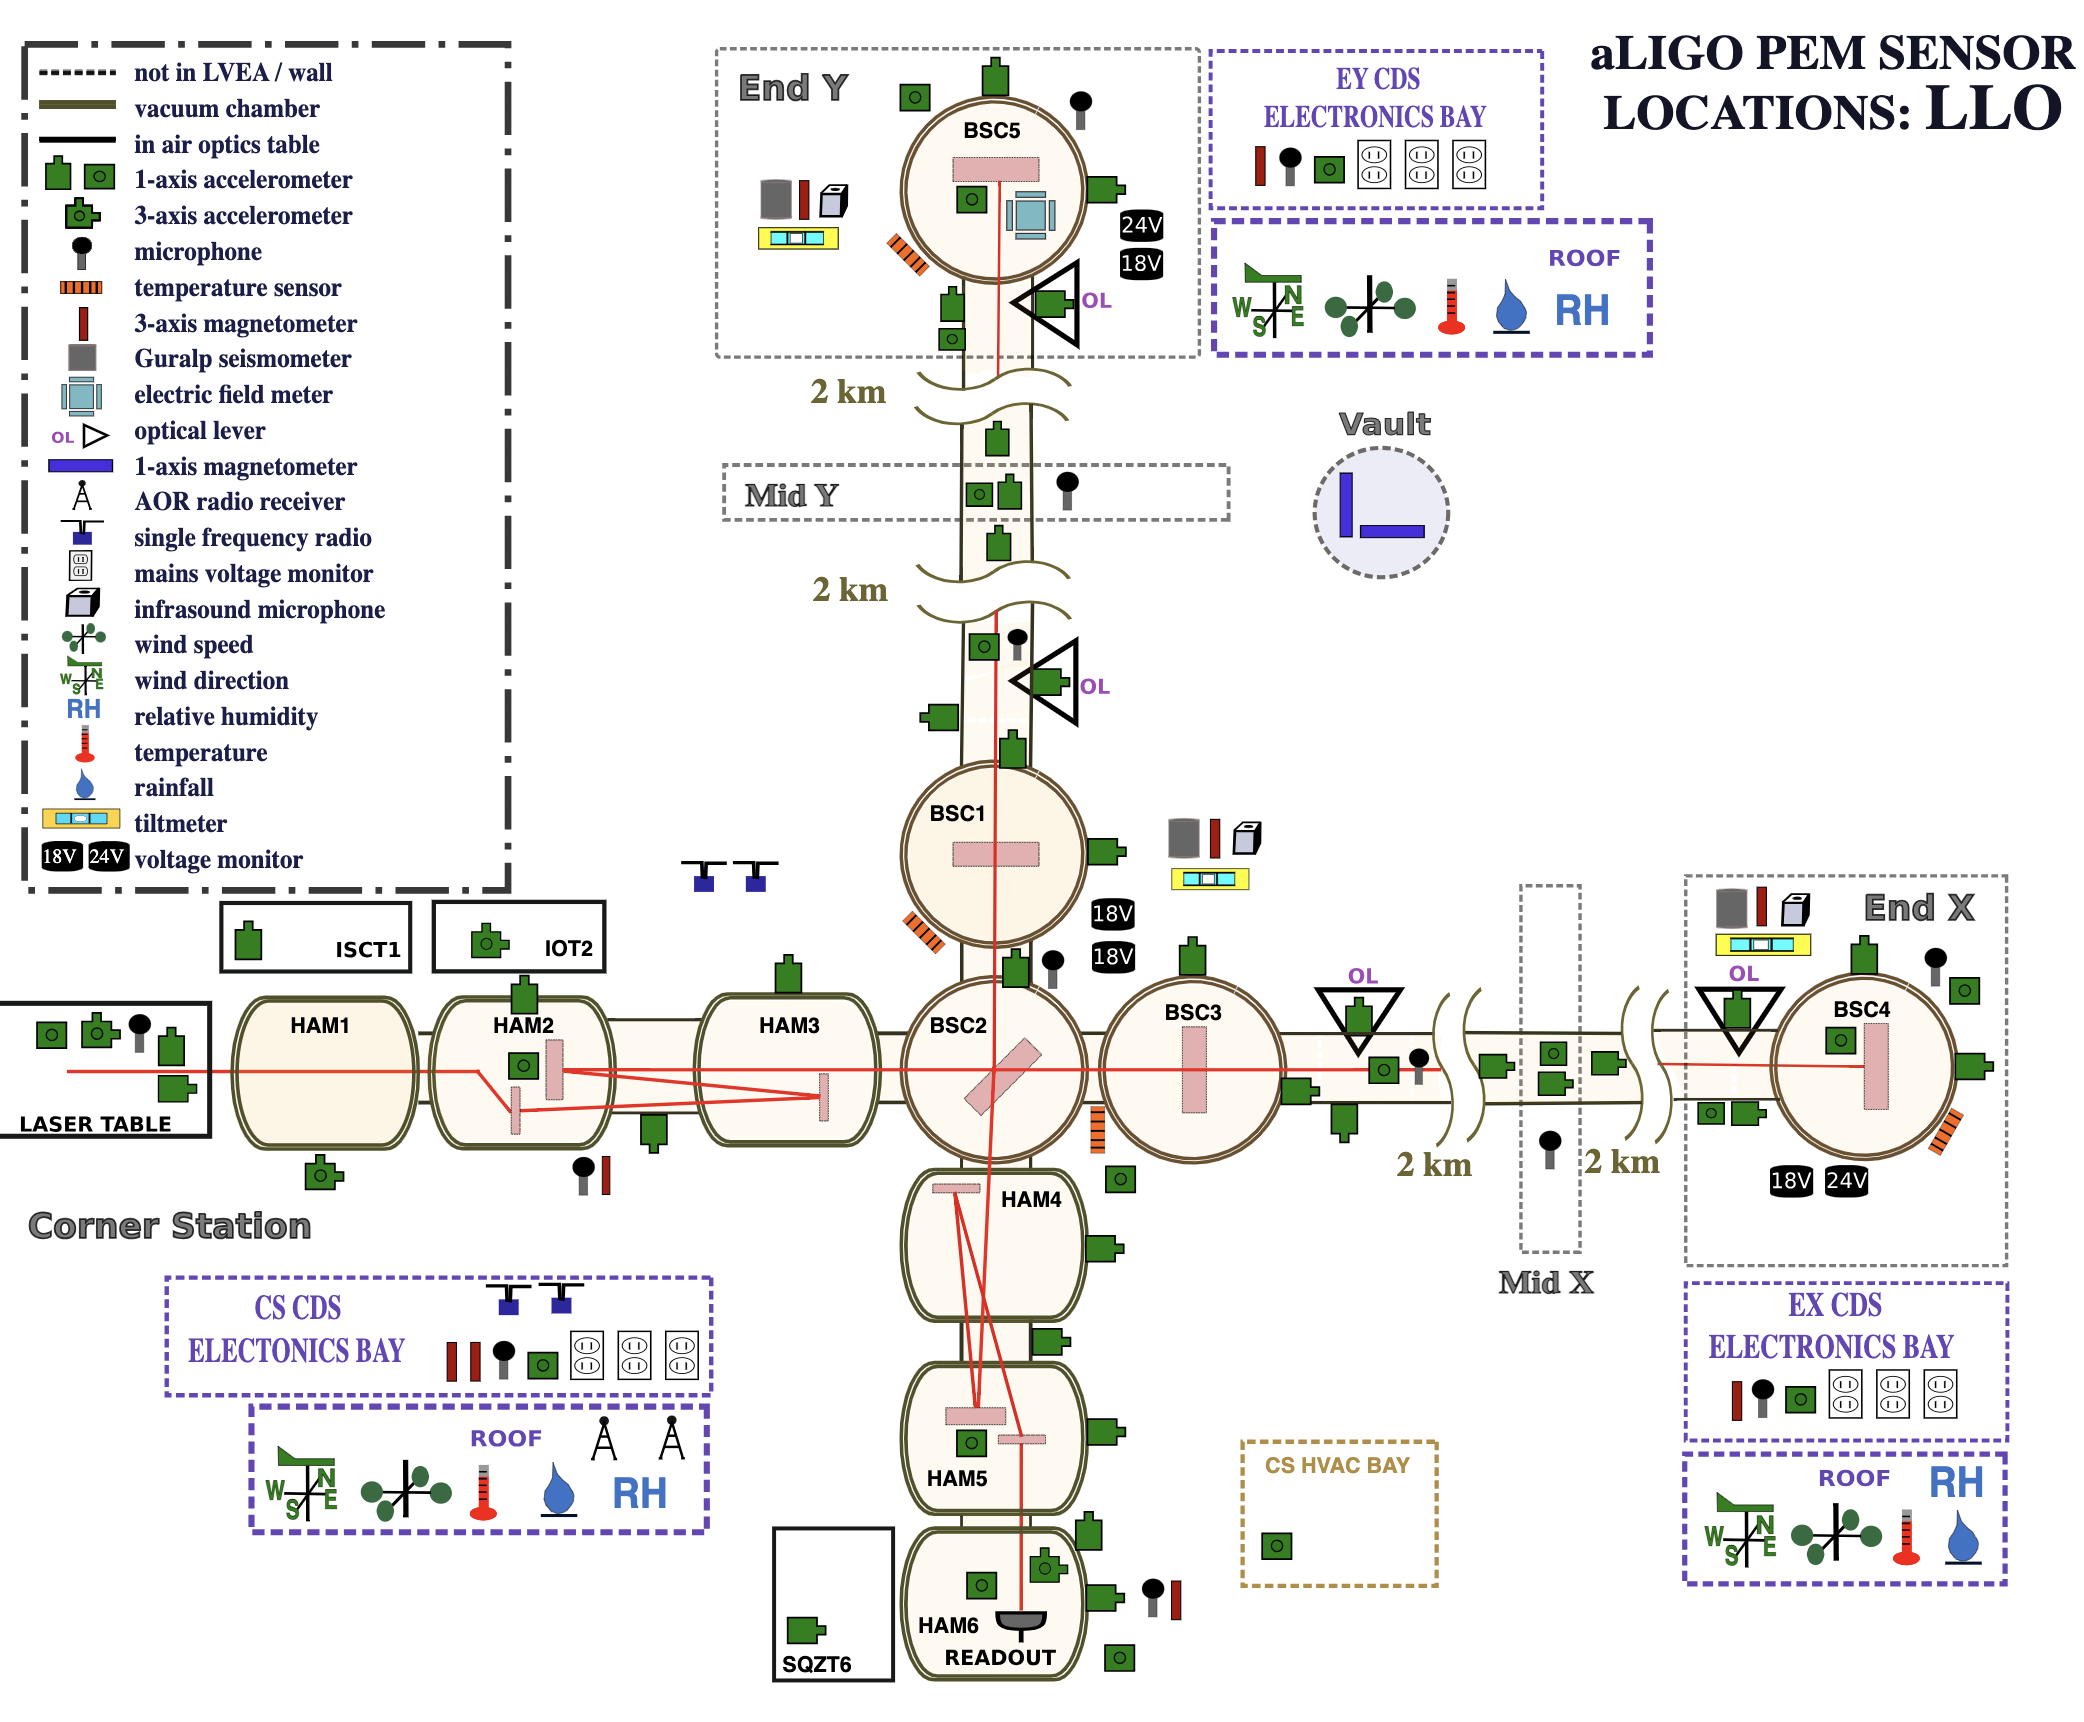
\includegraphics[width=1\columnwidth,height=1\columnwidth]{images/ligo_pem}
	\end{columns}		
	
	
	
				\extrafootertext{pem.ligo.org}
	
\end{frame}






\begin{frame}
	
	
	
	\begin{columns}
		\column{0.5\textwidth}
		
		\begin{itemize}
			\item Is the 60 Hz interference recorded by $r\,(t)$ also in $x(t)$?
			\item Coherence
			\begin{equation}
				C_{xr}(f)	= \frac{|P_{xr}(f\,)|^2}{P_{xx}(f\,) P_{rr}(f\,)}  \label{eq:coherence} \nonumber
			\end{equation}

		\end{itemize}
		
	
		\column{0.5\textwidth}
		\vspace*{-5mm}
		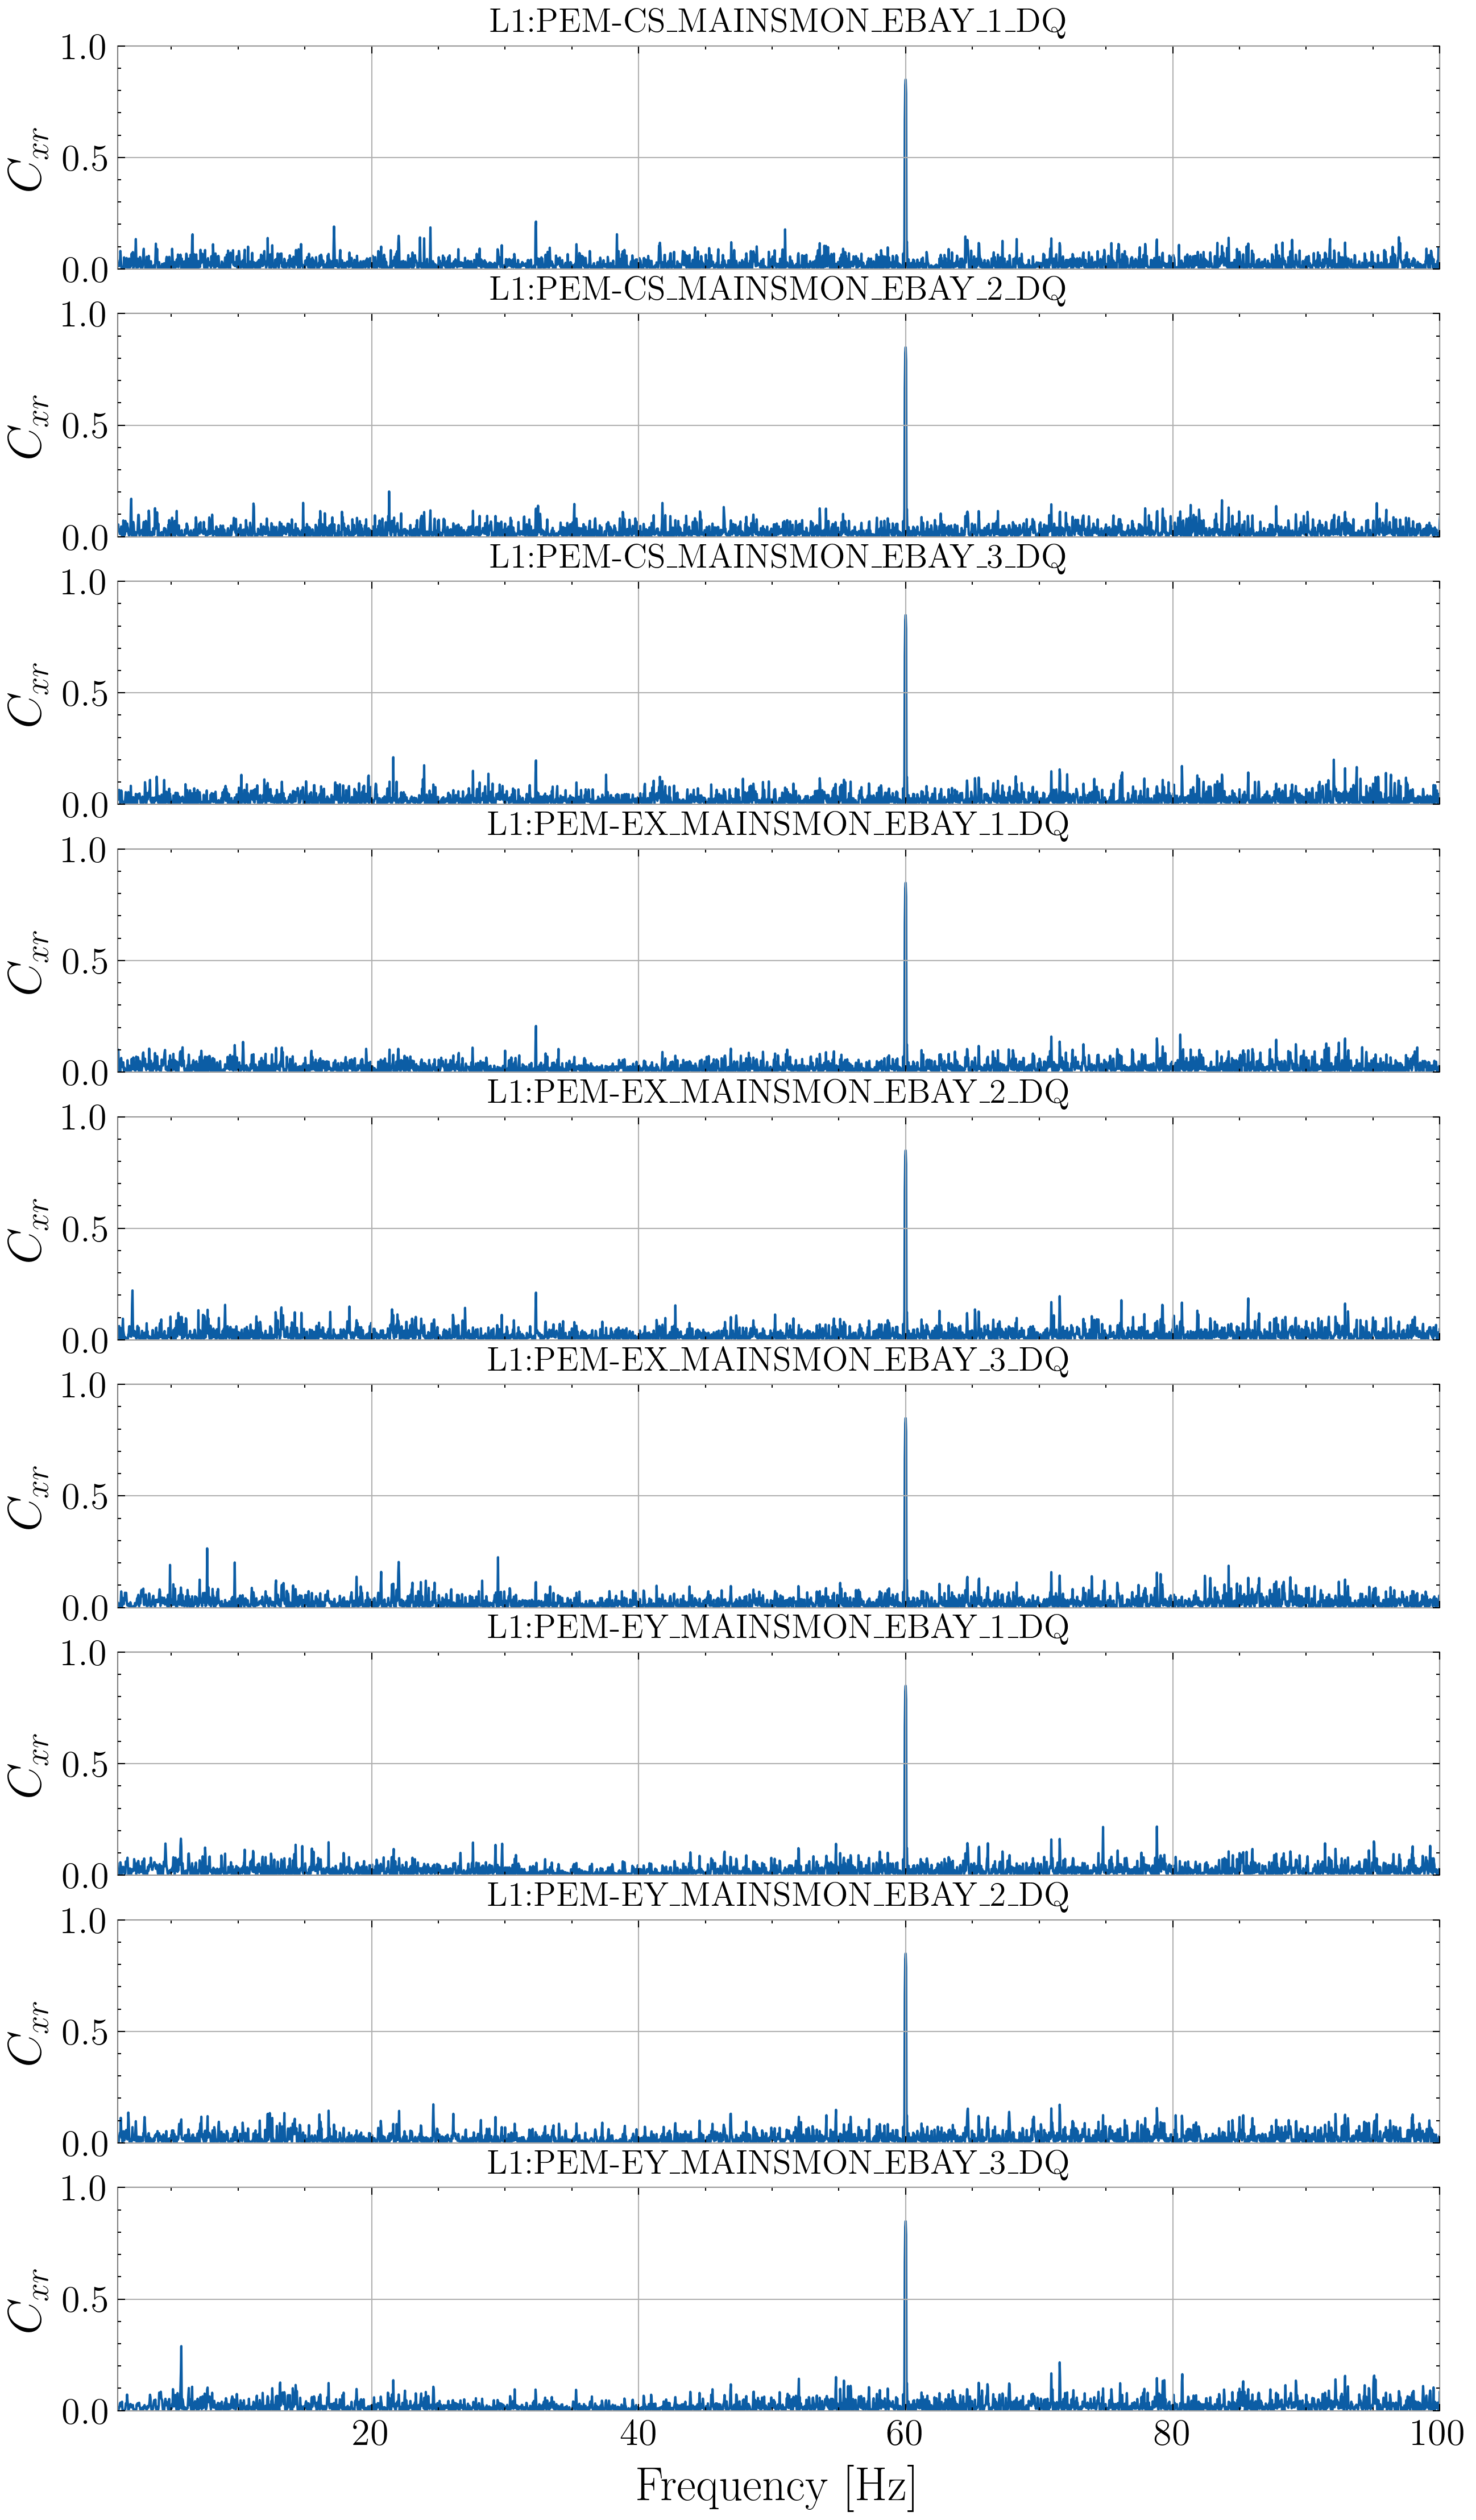
\includegraphics[width=0.82\columnwidth,height=1.5\columnwidth]{images/stacked_coherence_plot_new}
	\end{columns}		
	
\end{frame}




\begin{frame}{Validation with synthetic data}
	\alert{Goal}: Find a (wandering) CW signal that overlaps with the (wandering) 60 Hz interference line 
	
	
	Create some noisy synthetic data:
	$$x(t) = h(t) + c(t) + n(t) \, ; \,  r\,(t)$$
	

	Search for $h(t)$ using a HMM (\href{https://arxiv.org/abs/1606.02412}{Suvrova et al. 2016}) + ANC

\end{frame}



\begin{frame}
	
	\centering
			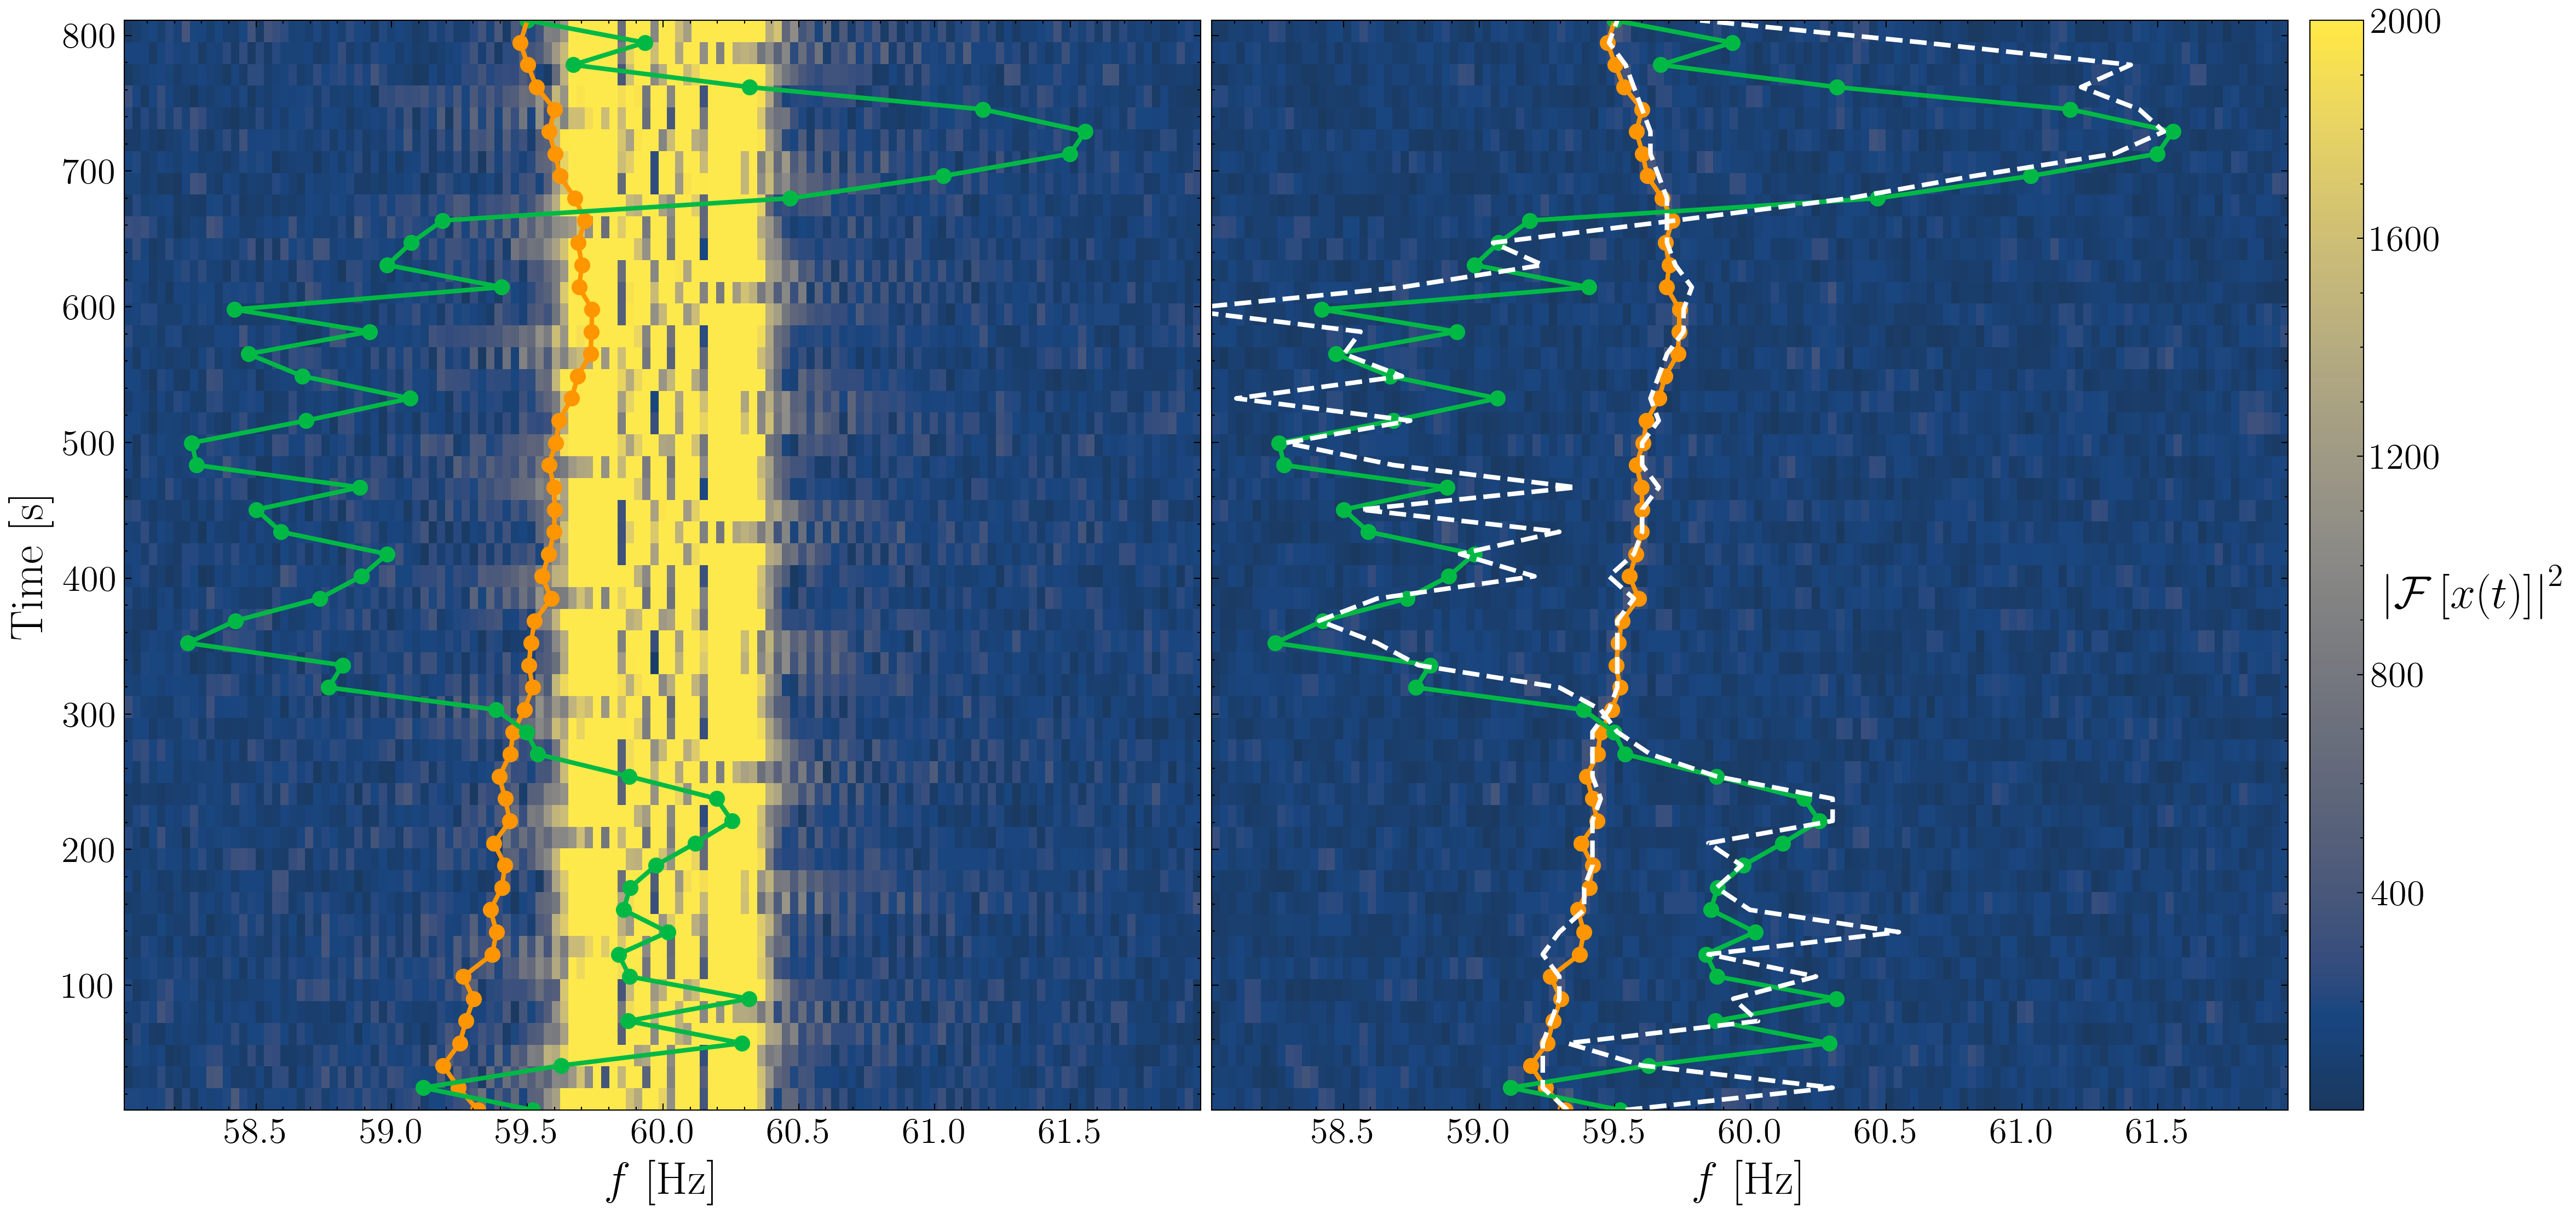
\includegraphics[width=1\textwidth,height=0.48\textwidth]{images/viterbi_tracking_canonical}
	
	

	
\end{frame}






	\begin{frame}{Summary}
	
	\metroset{block=fill}
	\begin{block}{\alert{Takeaway points}}
		\begin{itemize}
			\item Instrumental lines hamper CW searches.
			\item It is possible to subtract lines using adaptive noise cancellation (ANC) 
			\item ... if there is reference data from a PEM
			\item ANC + HMM search on synthetic data can recover CW signal which overlaps with mains power interference at 60 Hz
		\end{itemize}
	\end{block}
	
\end{frame}



%\begin{frame}[standout]
%	Appendices
%\end{frame}
%\appendix
%
%
%
%
%
%\begin{frame}{How is $c(t)$ modelled?}
%	Key properties of mains power:
%	\begin{enumerate}
%\item  Frequency is maintained at a constant value by internal grid mechanisms, i.e. a phase locked loop. A slow periodic modulation occurs about $f_{\rm ac}$ with period $P$ and amplitude $\Delta f_{\rm ac}$ , where the period wanders randomly
%\item Phase offset of the voltage wanders stochastically
%\item Voltage amplitude is random
%	\end{enumerate}
%
%	 \begin{align}
%		c(t) = A_r(t_n) \cos \left[ 2 \pi f_{\rm ac} t + \Theta(t)\right]
%		\label{eq:voltage}
%	\end{align}
%	with
%	\begin{eqnarray}
%		\Theta(t) = 2 \pi \Delta f_{\rm ac} \cos\left[\frac{2 \pi t}{P(t_n)}\right] + n_{\Theta} (t_n) \ ,
%		\label{eq:voltage_theta}
%	\end{eqnarray}
%	
%\end{frame}


	
\end{document}